\documentclass[letterpaper]{article}
\usepackage[margin=1in]{geometry}
\usepackage[utf8]{inputenc}
\usepackage{textcomp}
\usepackage{amssymb}
\usepackage{natbib}
\usepackage{graphicx}
\usepackage{gensymb}
\usepackage{amsthm, amsmath, mathtools}
\usepackage[dvipsnames]{xcolor}
\usepackage{enumerate}
\usepackage{mdframed}
\usepackage[most]{tcolorbox}
\usepackage{csquotes}
% https://tex.stackexchange.com/questions/13506/how-to-continue-the-framed-text-box-on-multiple-pages

\tcbuselibrary{theorems}

\newcommand{\R}{\mathbb{R}}
\newcommand{\Z}{\mathbb{Z}}
\newcommand{\N}{\mathbb{N}}
\newcommand{\Q}{\mathbb{Q}}
\newcommand{\C}{\mathbb{C}}
\newcommand{\code}[1]{\texttt{#1}}
\newcommand{\mdiamond}{$\diamondsuit$}
\newcommand{\PowerSet}{\mathcal{P}}
\newcommand{\Mod}[1]{\ (\mathrm{mod}\ #1)}
\DeclareMathOperator{\lcm}{lcm}

%\newtheorem*{theorem}{Theorem}
%\newtheorem*{definition}{Definition}
%\newtheorem*{corollary}{Corollary}
%\newtheorem*{lemma}{Lemma}
\newtheorem*{proposition}{Proposition}


\newtcbtheorem[number within=section]{theorem}{Theorem}
{colback=green!5,colframe=green!35!black,fonttitle=\bfseries}{th}

\newtcbtheorem[number within=section]{definition}{Definition}
{colback=blue!5,colframe=blue!35!black,fonttitle=\bfseries}{def}

\newtcbtheorem[number within=section]{corollary}{Corollary}
{colback=yellow!5,colframe=yellow!35!black,fonttitle=\bfseries}{cor}

\newtcbtheorem[number within=section]{lemma}{Lemma}
{colback=red!5,colframe=red!35!black,fonttitle=\bfseries}{lem}

\newtcbtheorem[number within=section]{example}{Example}
{colback=white!5,colframe=white!35!black,fonttitle=\bfseries}{def}

\newtcbtheorem[number within=section]{note}{Important Note}{
        enhanced,
        sharp corners,
        attach boxed title to top left={
            xshift=-1mm,
            yshift=-5mm,
            yshifttext=-1mm
        },
        top=1.5em,
        colback=white,
        colframe=black,
        fonttitle=\bfseries,
        boxed title style={
            sharp corners,
            size=small,
            colback=red!75!black,
            colframe=red!75!black,
        } 
    }{impnote}
\usepackage[utf8]{inputenc}
\usepackage[english]{babel}
\usepackage{fancyhdr}
\usepackage[hidelinks]{hyperref}

\pagestyle{fancy}
\fancyhf{}
\rhead{CSE 101}
\chead{Monday, February 28, 2022}
\lhead{Lecture 21}
\rfoot{\thepage}

\setlength{\parindent}{0pt}

\begin{document}

\section{Dynamic Programming}
We continue our discussion on dynamic programming. 

\subsection{Problem: Maximum Independent Set of Trees}

\begin{definition}{Independent Set}{}
    In an undirected graph $G$, an \textbf{independent set} is a subset of the vertices of $G$, no two of which are connected by an edge.
\end{definition}
For example, the following is an independent set:
\begin{center}
    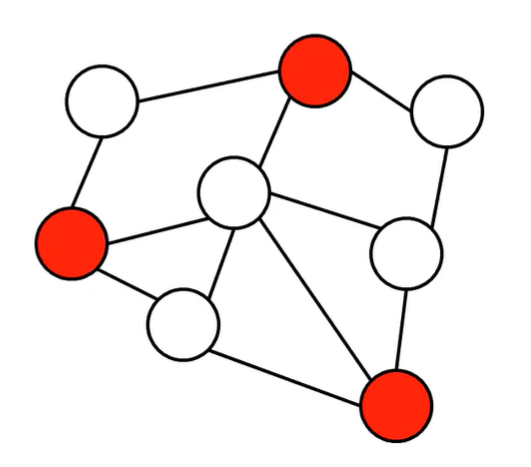
\includegraphics[scale=0.3]{../assets/ind_set.png}
\end{center}

\textbf{Problem Statement:} Given an undirected graph $G$, compute the largest possible \textbf{size} of an independent set of $G$. 

\bigskip 

Call the result of the largest possible independent set $I(G)$; in the example above, $I(G) = 3$. 


\subsubsection{Simple Recursion}
\begin{center}
    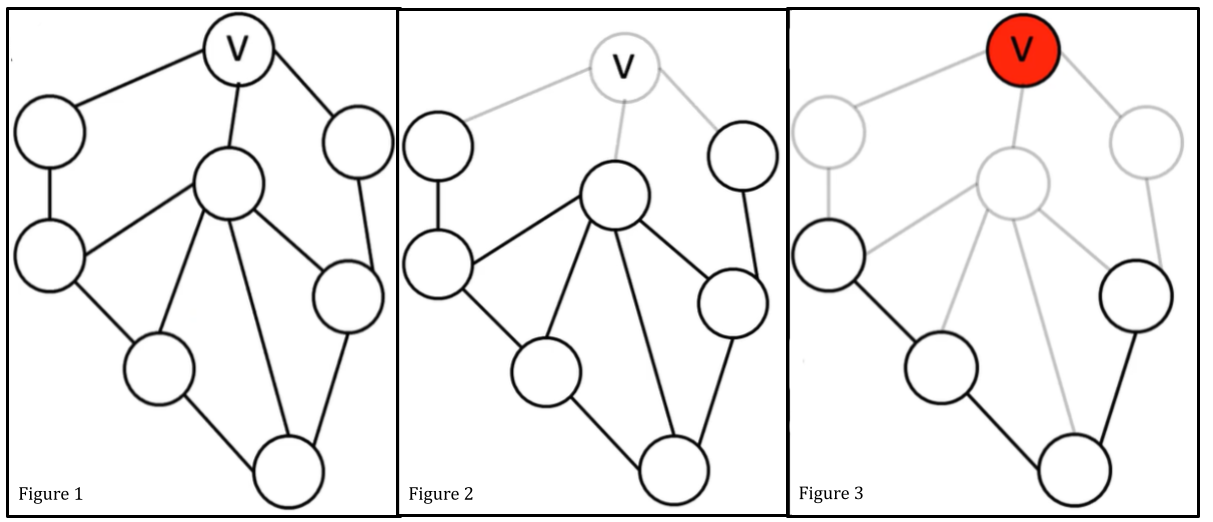
\includegraphics[scale=0.35]{../assets/ind_set_ex.png}
\end{center}

There is a reasonably simple recursion that can be used here. A simple question we can ask is: \emph{is vertex $v$ in the independent set?} We'll consider Figure 1 above as a baseline example.
\begin{itemize}
    \item If $v$ is not in the independent set, then the maximum independent set is an independent set of $G \setminus \{v\}$. In other words, we have 
    \[I(G) = I(G \setminus \{v\})\]
    For example, Figure 2 shows what this could look like.
    \item If so, then the maximum independent set is $v$ plus an independent set of $G \setminus N(v)$, where $N(v)$ denote the set of vertices which are neighbors of $v$. In other words, we have 
    \[I(G) = 1 + I(G \setminus N(v))\]
    For example, Figure 3 shows what this could look like.
\end{itemize}
Therefore, our recursion can be defined by 
\[I(G) = \max(I(G \setminus \{v\}), 1 + I(G \setminus N(v)))\]


\subsubsection{Subproblems}
We now consider the subproblems generated by this recursion. 
\begin{center}
    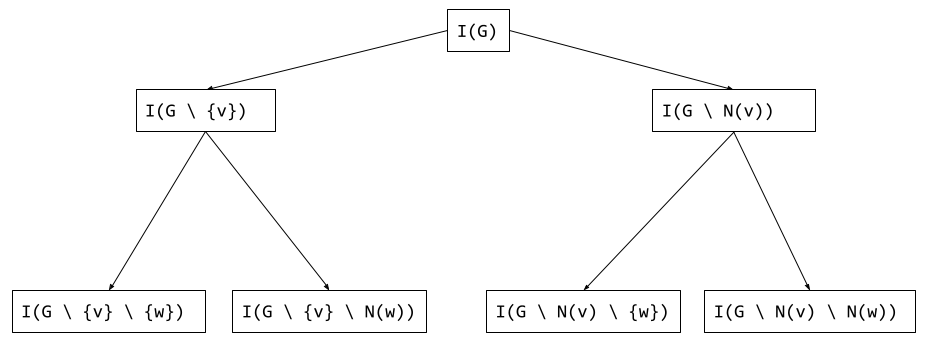
\includegraphics[scale=0.5]{../assets/indep_set_sub.png}
\end{center}
Here, it's not hard to see that, if we continued generating this recursion tree, we see very little subproblem reuse. In other words, we end up with \emph{different subproblems} every time we get a new recursion. This is an issue for dynamic programming, as dynamic programming relies on subproblem reusability for efficiency.  

\bigskip 

In particular, for every subgraph $G'$, we need subproblems $I(G')$. But, we'll end up with $2^{|V|}$ subproblems; each vertex can either be in $G'$ or it can not be in $G'$. This further implies that the runtime of this algorithm will be exponential. 

\subsubsection{Hardness}
Maximum Independent Set of any general graph is what is known as an \textbf{NP-Hard} problem. Basically, this means that people believe that there may well be no \emph{efficient} algorithm for it (there is no sub-exponential runtime algorithm that solves this problem). 

\bigskip 

Instead, we now consider \emph{special cases} of this problem where we can do better. 

\subsubsection{Independent Sets and Components}
\begin{lemma}{}{}
    If $G$ has connected components $C_1, C_2, \dots, C_k$, then 
    \[I(G) = I(C_1) + I(C_2) + \dots + I(C_k)\]
\end{lemma}
\begin{mdframed}[]
    \begin{proof}
        Since the components don't connect to each other, an independent set for $G$ is exactly the union of an independent set for each of the $C_i$'s. THen, we can pick the biggest set for each $C_i$. 
    \end{proof}
\end{mdframed}

\subsubsection{Independent Sets of Trees}
One special case we can consider is independent sets of \emph{trees}. The reason why we look at trees is because, when we remove vertices from trees, it splits the tree up into disconnected subgraphs. This is useful as we can consider the disconnected subgraphs separately.
\begin{center}
    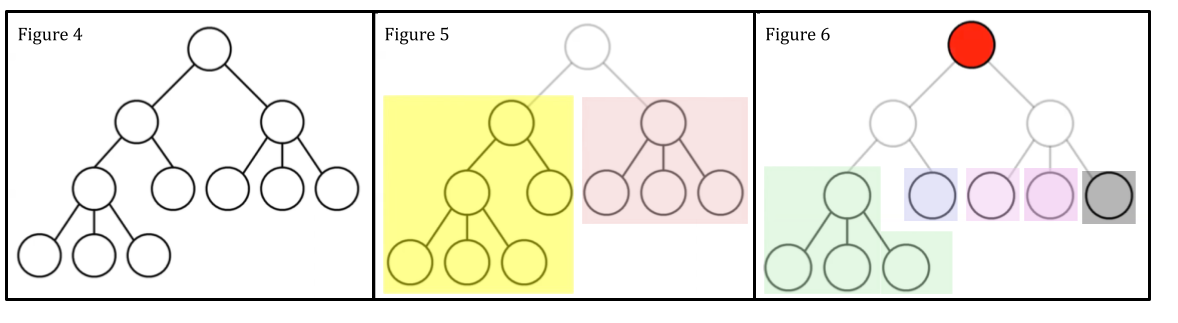
\includegraphics[scale=0.35]{../assets/indep_set_tree.png}
\end{center}
Consider the above tree (Figure 4), and suppose we're focusing on the root of this tree $r$.
\begin{itemize}
    \item If we do \emph{not} include $r$ in our maximum independent set, then we want to look at the maximum independent sets of $G \setminus \{r\}$. For this, see Figure 5. 
    \item If we \emph{do} include $r$ in our maximum independent set, then we get $r$ for free, remove all of the neighbors of $r$, and then we can consider the remaining subgraphs. For this, see Figure 6. 
\end{itemize}
We note that the subproblems here are actually all \emph{sub-trees} of the original tree. If we look at a subtree of a subtree, we note that this is simply just another subtree. Then, it follows that the set of all problems that we need to solve is just the set of all possible subtrees of the original tree. 

\subsubsection{Recursion of the Tree}
We now consider several cases for our tree. 
\begin{itemize}
    \item Suppose the root is not used in the tree. Then, we end up with the subproblem of having to find the sum of the maximum independent sets of all of the children subtrees. That is, 
    \[I(G) = \sum I(\text{Children's Subtrees})\]
    This is shown by Figure 7 below.

    \item Suppose the root is used. Then, we end up with the subproblem of having to find the sum of all of the maximum independent sets of all of the grandchildren subtrees. That is, 
    \[I(G) = 1 + \sum I(\text{Grandchildren's Subtrees})\]
    This is shown by Figure 8 below.
\end{itemize}

\begin{center}
    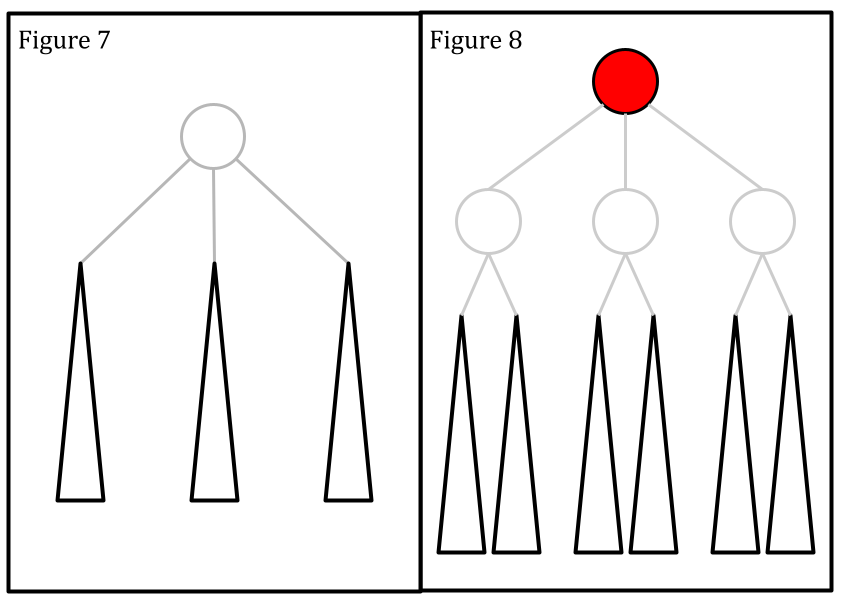
\includegraphics[scale=0.4]{../assets/indep_set_trees_2.png}

    \textbf{Note:} Triangles are arbitrary subtrees. 
\end{center}


\subsubsection{Example: Computing Maximum Independent Set of Trees}
Consider the following tree: 
\begin{center}
    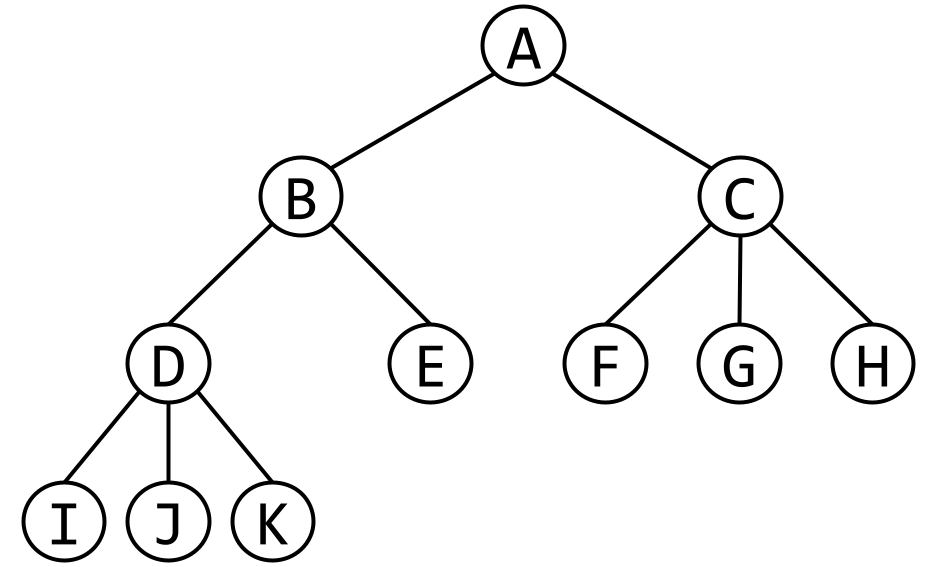
\includegraphics[scale=0.3]{../assets/ind_set_ex_tree.png}
\end{center}
Compute the maximum independent set. 

\begin{mdframed}[]
    Remember, our subproblems are the subtrees. So, for each node, we associate that node to the subproblem that corresponds to what is the maximum independent set of that node's subtree. The formula that we have is that this will always be the maximum of either: 
    \begin{itemize}
        \item The sum of the children's answers. 
        \item One more than the sum of the grandchildren's answers.
    \end{itemize}

    So, we start at the leaves and make our way up. 
    \begin{itemize}
        \item At the bottom level, each leaf (I, J, K, E, F, G, H) is going to have an answer of 1. If we just have that single node, the biggest independent set is going to be of size 1.
        \begin{center}
            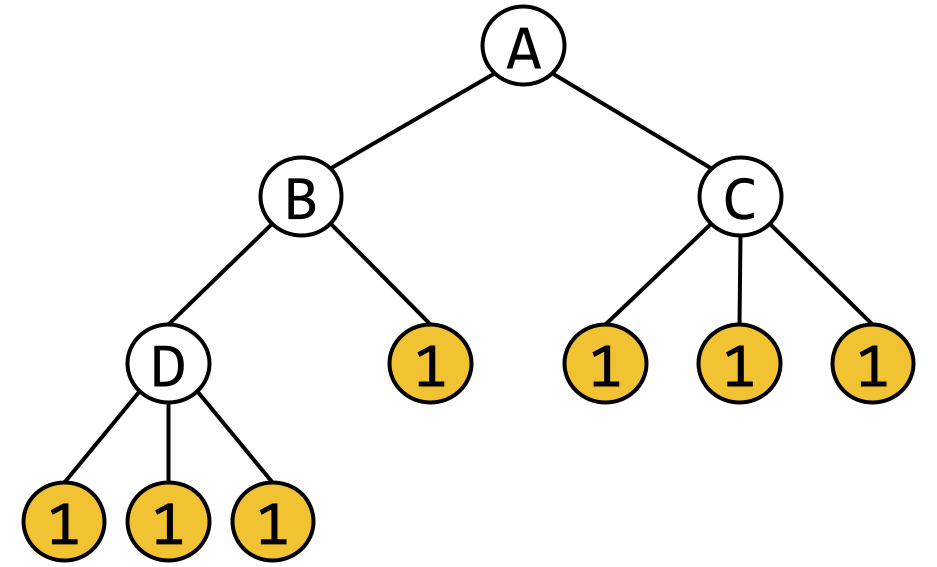
\includegraphics[scale=0.2]{../assets/indep_set_ex_1.png}
        \end{center}

        \item Consider node $D$. We can either take the sum of the children ($1 + 1 + 1 = 3$) or we can take one plus the sum of the grandchildren ($1 + 0 = 1$). Clearly, the sum of the children is the best option, so $D$ will be 3. 
        \begin{center}
            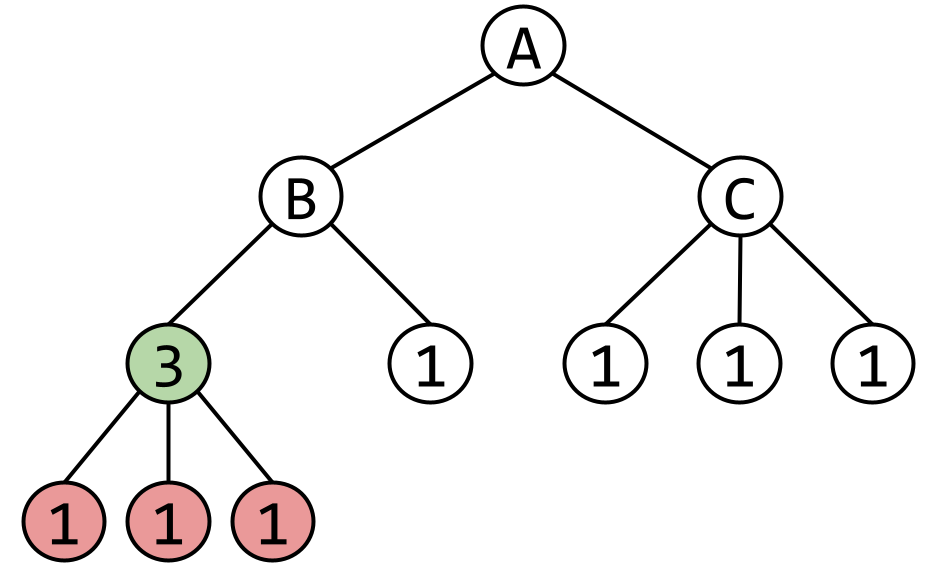
\includegraphics[scale=0.2]{../assets/indep_set_ex_2.png}
        \end{center}
        Note that the children nodes are \emph{red} while node $D$ is \emph{green}.

        \item Consider node $B$. We can either take the sum of the children ($3 + 1 = 4$) or we can take one plus the sum of the grandchildren ($1 + (1 + 1 + 1) = 4$). Both options are good, so $B$ will be 4. 
        \begin{center}
            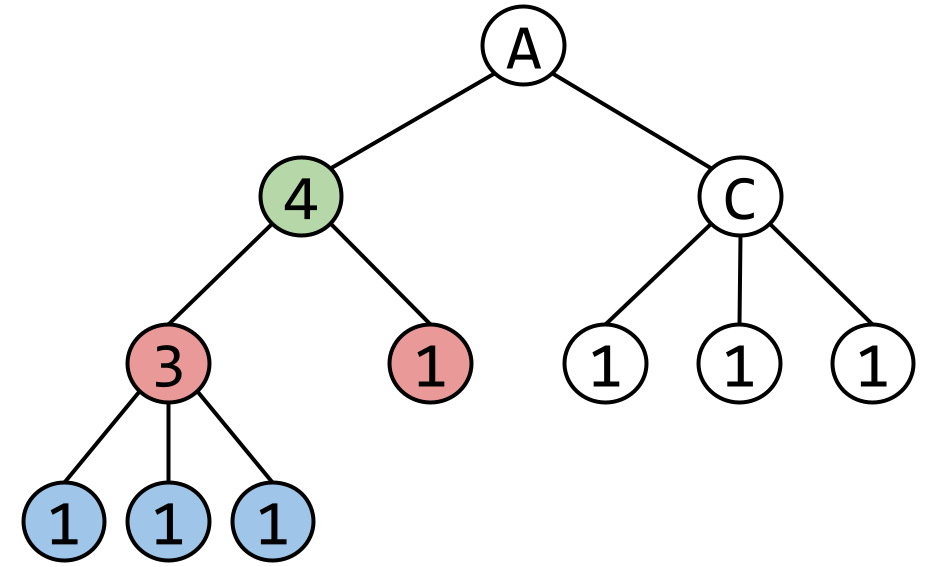
\includegraphics[scale=0.2]{../assets/indep_set_ex_3.png}
        \end{center}
        Note that the children nodes are \emph{red}, the grandchildren nodes are \emph{blue}, and node $B$ is \emph{green}.

        \item Consider node $C$. We can either take the sum of the children ($1 + 1 + 1 = 3$) or we can take one plus the sum of the grandchildren ($1 + 0 = 1$). Clearly, the sum of the children is the best option, so $C$ will be 3. 
        \begin{center}
            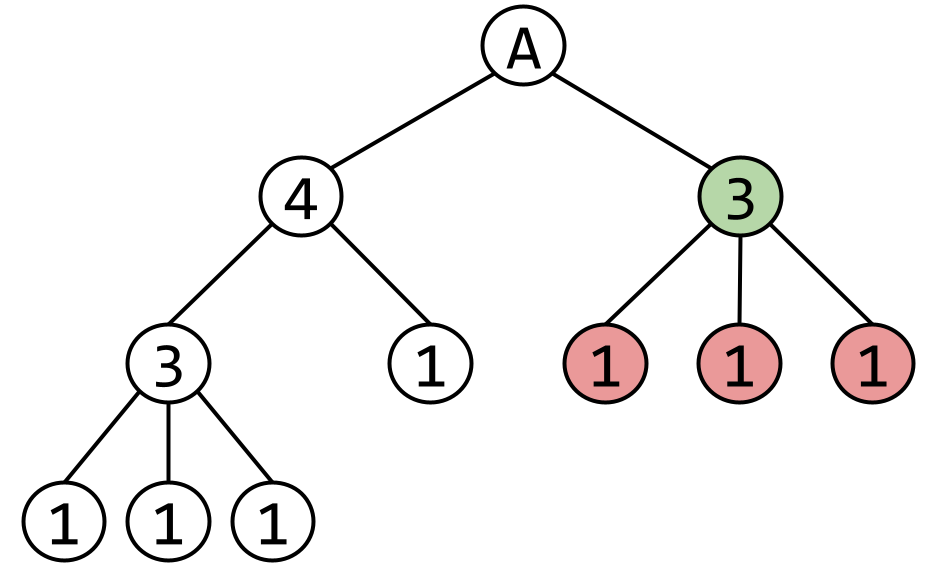
\includegraphics[scale=0.2]{../assets/indep_set_ex_4.png}
        \end{center}
        Note that the children nodes are \emph{red} and node $C$ is \emph{green}. Additionally, note that this is actually a subproblem that we've seen before.

        \item Consider node $A$. We can either take the sum of the children ($4 + 3 = 7$) or we can take one plus the sum of the grandchildren ($1 + (3 + 1 + 1 + 1 + 1) = 8$). Clearly, one plus the sum of the grandchildren is the best option, so $A$ will be 8. 
        \begin{center}
            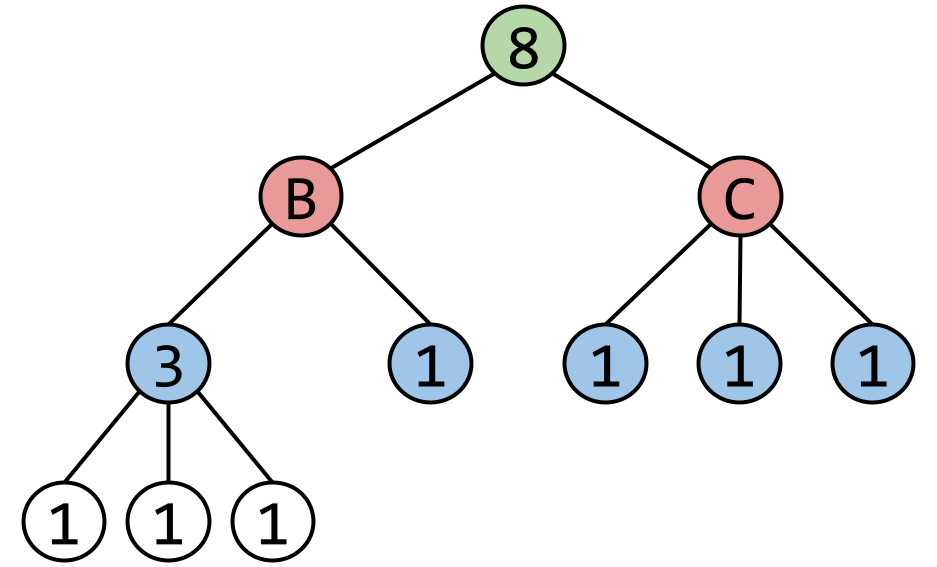
\includegraphics[scale=0.2]{../assets/indep_set_ex_5.png}
        \end{center}
        Note that the children nodes are \emph{red}, the grandchildren nodes are \emph{blue}, and node $A$ is \emph{green}.
    \end{itemize}
    Therefore, the maximum independent set of the \emph{whole tree} is \boxed{8}.
\end{mdframed}


\subsection{Problem: Traveling Salesman Problem}
\emph{In your job as a door-to-door vacuum salesperson, you need to plan a route that takes you through $n$ different cities. In order to space things out, you do not want to get back to the start until you have visited all cities. You also want to do so with as little travel as possible. }

\bigskip 

\textbf{Problem Statement:} Given a weighted (undirected) graph $G$ with $n$ vertices, find a cycle that visits each vertex exactly once whose total weight is as small as possible.


\subsubsection{Naive Algorithm}
The naive algorithm is to try all possible paths and see which is the cheapest. There are $n!$ paths; in particular, if we assume that we have a complete graph where all edges are there, then: 
\begin{itemize}
    \item There are $n$ possible options for the first city.
    \item There are $n - 1$ possible options for the second city. 
    \item There are $n - 2$ possible options for the third city. 
    \item \dots
\end{itemize}
This gives us $n(n - 1)(n - 2) \dots (2)(1) = n!$. Therefore, the runtime of the naive algorithm is approximately $\BigO(n!)$. 

\subsubsection{Problem Difficulty}
Like Maximum Independent Set, the Traveling Salesman Problem is widely considered to be a difficult problem. It is widely believed that there is no polynomial time algorithm for it. That being said, we note that there is an algorithm that beats the $n!$ naive algorithm.

\subsubsection{Setup}
We need to find some notion of \emph{partial solutions} for subproblems. In our case of cycles, we want to look for a path from vertex $s$ to $t$ such that, by adding one more vertex, we get a cycle. Therefore, the answer is given by 
\[\text{Best}_{st}(G) = \ell(s, t)\]
where $\text{Best}_{st}(G)$ is the best value of a path starting at vertex $s$ and ending at vertex $t$ that visits each vertex exactly once. 

\subsubsection{Recursion}
Suppose we have this path from $s$ to $t$. 
\begin{center}
    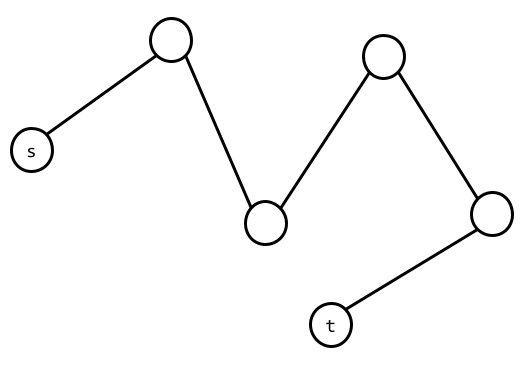
\includegraphics[scale=0.4]{../assets/st_path_1.png}
\end{center}
We need to find some recursion that relates the answer to this problem to some kind of subproblem. The standard way to do this is to ask ourselves: what happens if we undo the last step? In our case, our last step is some edge from $u$ to $t$. That is: 
\begin{center}
    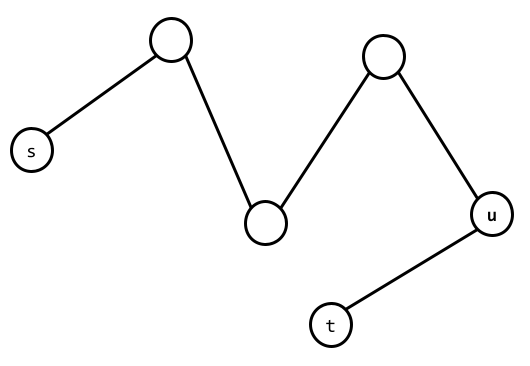
\includegraphics[scale=0.4]{../assets/st_path_2.png}
\end{center}
The weight is, then, given by 
\[\ell(u, t) + \text{Length of Rest of Path}\]
We want the best path from $s$ to $u$ that uses every vertex \emph{except for $t$}. 
\begin{center}
    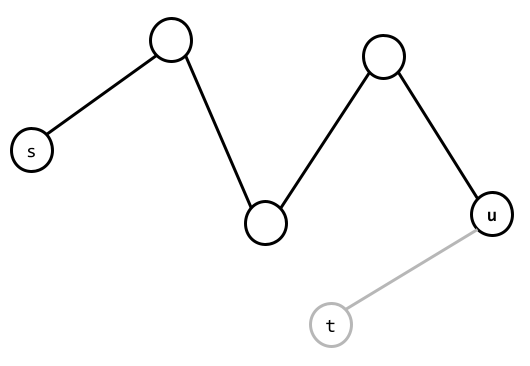
\includegraphics[scale=0.4]{../assets/st_path_3.png}
\end{center}
Let's call this subproblem $\text{Best}_{su, -t}$; this is the minimum weight of the path from $s$ to $u$ that visits every vertex except for $t$ exactly once. Thus, the formula is given by 
\[\text{Best}_{st}(G) = \min_{u} \left(\text{Best}_{su, -t}(G) + \ell(u, t)\right)\]
For each $t$, we figure out what the best path is, add the length of the edge from $u$ to $t$, and then we take the minimum over all the possible vertices $u$ that have an edge to $t$. This will give us the best possible path length from $s$ to $t$. 

\subsubsection{Recursion II}
Now that we have a recursion that gives us the final answers in terms of subproblems, but we need a recursion that solves the subproblems. In other words, how do we solve for $\text{Best}_{su, -t}(G)$? 

\bigskip 

Again, we look at the edge from $v$ to $u$. We need the best path that connects $s$ to $v$ that uses all vertices except for $t$ and $u$. However, this makes the subproblems more complicated; all we're doing is avoiding more vertices. 

\bigskip 

Instead, we define $\text{Best}_{st, L}$ to be the best path length from $s$ to $t$ that uses exactly the vertices in $L$. That is, every vertex in $L$ shows up in the path exactly once. The rest of the vertices not in $L$ do not show up in the path. 

\bigskip 

The last edge is some $(v, t) \in E$ for some $v \in L$. Then, the cost of the path is given by 
\[\text{Best}_{sv, L \setminus \{t\}} + \ell(v, t)\]
So, the full recursion is given by 
\[\text{Best}_{st, L}(G) = \min_v \left(\text{Best}_{sv, L \setminus \{t\}}(G) + \ell(v, t)\right)\]

\subsubsection{Runtime Analysis}
Note that $L$ can be any subset of the vertices; thus, there are $2^n$ possibilities. Additionally, $s$ and $t$ can both be any vertices; thus, there are $n^2$ possibilities. Thus, there are $n^2 2^n$ subproblems. 

\bigskip 

We also need to check this for every $v$ (every vertex). This is because, for each subproblem, we need to find the minimum out of all vertices $v$. Thus, each subproblem takes $\BigO(n)$ time. 

\bigskip 

The final runtime is then given by $\BigO(n^3 2^n)$. 

\end{document}